\chapter{Resultados}\label{resultados}

Os resultados vem aqui.

\section{Simulação}\label{resultadosSimulacao}

É possível criar seções e subseções dentro do documento. Isso vai deixar o trabalho mais organizado.




\subsection{Simulação Particular}\label{resultadosSimulacao_sub}

Escreva neste local resultados particulares de alguma simulação realizada, caso isso seja necessário.



\section{Aplicação}\label{aplicacao}

Aplicação a dados reais do método descrito no Capítulo \ref{modelagem}. A Figura \ref{serietemporal} mostra os dados analisados neste trabalho. 


\begin{figure}[!h]
\centering
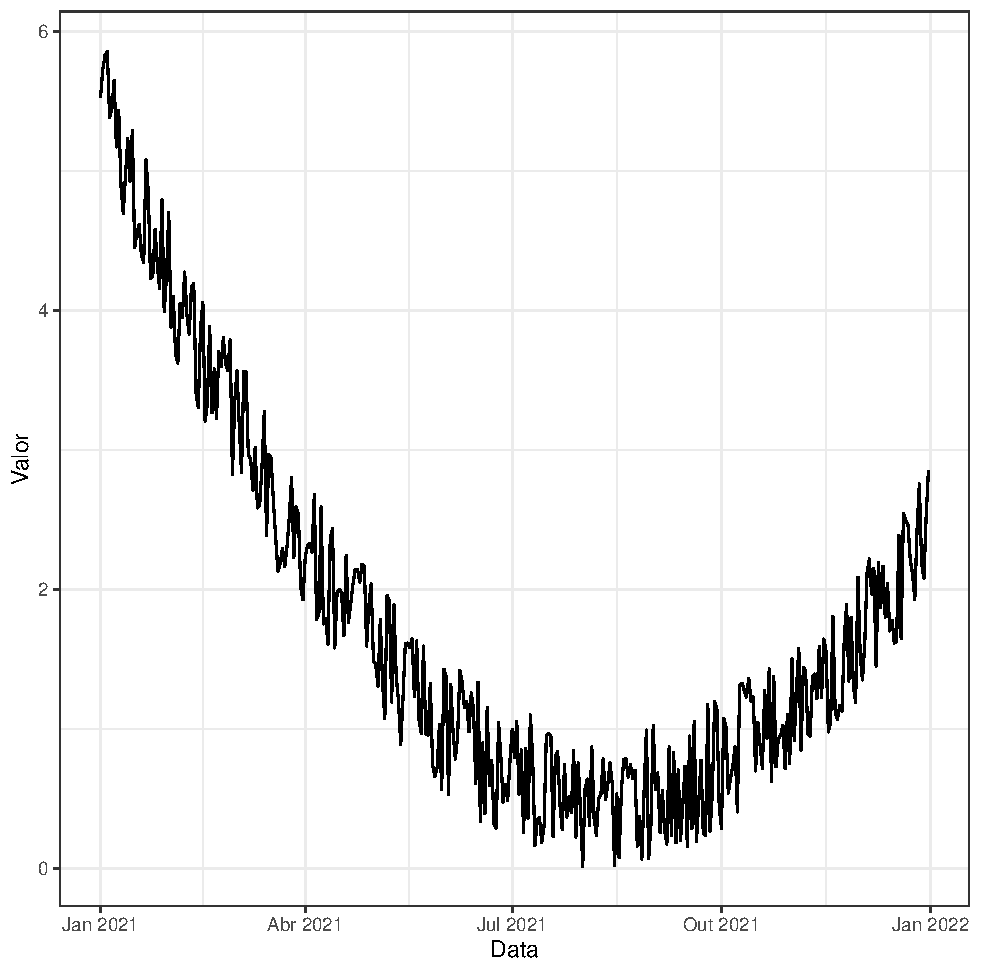
\includegraphics[width=0.8\textwidth]{figuras/serie_temporal.pdf}
\label{serietemporal}
\end{figure}


Devido a características do próprio LaTeX, as figuras podem acabar ficando em posições estranhas às vezes. Em geral, quanto mais texto for escrito, mais fácil é para o programa encontrar locais mais adequados para as figuras.


\marcus{Este comando é interessante. Ele está definido na linha 186 do arquivo 00-Monografia.tex.}{Com este comando, é possível o orientador fazer comentários mais efetivos na correção do texto do aluno, caso ambos estejam usando o Overleaf para trabalhar.}
